\documentclass[12pt,a4paper,oneside,onecolumn]{article}

\usepackage[spanish,es-noshorthands]{babel}
\usepackage{epsfig}
\usepackage[latin1]{inputenc}
\usepackage{amsmath}
\usepackage{amsfonts}
\usepackage{amssymb}
%\usepackage{mathabx}  Compila pero borra el pdf?
\usepackage{array}
\usepackage[left=1.8cm, right=1.8cm, top=2.50cm, bottom=2.5cm]{geometry}
\usepackage{hyperref}
\usepackage{color}
\usepackage{fancyhdr}
\usepackage{listings}
\usepackage{xcolor}
\usepackage[smartEllipses]{markdown}

\pagestyle{fancy}

\fancyhead{}
\fancyfoot{}

\setlength{\headsep}{0.4cm}
\setlength{\footskip}{1.6pt}
\setlength{\parindent}{0pt}
\setlength{\extrarowheight}{1.5pt}


\lhead{Proyectos II}
\rhead{Javier Orti}
\renewcommand*\headrulewidth{0.4 pt}
\lfoot{\vspace{0.45cm}File Inclusion}
\cfoot{\vspace{0.01cm}\rule{\linewidth}{0.4pt}}
\rfoot{\vspace{0.45cm} P\'ag. \thepage}

\renewcommand{\labelitemi}{$\bullet$}
\renewcommand{\labelenumi}{\theenumi)}
\renewcommand\spanishtablename{Tabla}

\decimalpoint

\headheight 16.7pt 
\textheight 715pt 

\parskip 8pt  

\hypersetup{
	colorlinks=true,
	linkcolor=blue,
	filecolor=magenta,      
	urlcolor=cyan,
}

% Python code settings
\definecolor{codegreen}{rgb}{0,0.6,0}
\definecolor{codegray}{rgb}{0.5,0.5,0.5}
\definecolor{codepurple}{rgb}{0.58,0,0.82}
\definecolor{backcolour}{rgb}{0.95,0.95,0.92}

\lstdefinestyle{mystyle}{
	backgroundcolor=\color{backcolour},   
	commentstyle=\color{codegreen},
	keywordstyle=\color{magenta},
	numberstyle=\tiny\color{codegray},
	stringstyle=\color{codepurple},
	basicstyle=\ttfamily\footnotesize,
	breakatwhitespace=false,         
	breaklines=true,                 
	captionpos=b,                    
	keepspaces=true,                 
	numbers=left,                    
	numbersep=5pt,                  
	showspaces=false,                
	showstringspaces=false,
	showtabs=false,                  
	tabsize=2
}

\lstset{style=mystyle}

\usepackage[shortlabels]{enumitem}
\usepackage{cancel}

\begin{document} 
    \section{}
    La vulnerabilidad de file inclusion consiste en aprovechar que el servidor incluye archivos locales o remotos en un script para que en su lugar el atacante intente acceder a otras partes del sistema o a archivos externos ya preparados.
    \section{}
    as
    \section{}
    \begin{enumerate}[]
        \item
        \underline {Local:} El script incluye archivos internos del sistema, por lo que el delincuente, si la aplicaci\'on tiene un mal dise\~no, podr\'ia acceder a otras partes del sistema, incluso a zonas de superuser.
        \item
        \underline {Remoto:} El script incluye archivos mediante una URL externa, por lo que si esta URL se pudiese modificar, en principio se podr\'ia incluir cualquier script externo malicioso e introducirlo en la m\'aquina de la v\'ictima.
    \end{enumerate}
    \section{}
    El filtro m\'as importante podr\'ia ser escribir a 'fuego' los archivos que el script va a incluir, de esa forma no da pie a modificaciones. Pero como en muchos casos vamos a requerir inclusiones din\'amicas, podremos optar por validar el input del usuario.
    Una medida sencilla pero bastante efectiva es por ejemplo solo permitir caracteres alfanum\'ericos y prohibir el resto.
    Si usamos PHP, es importante tener muy en cuenta la configuraci\'on de require, require\_once, include, include\_once
    \section{}
    Un ejemplo que ya hemos mencionado en otros retos, es introducir null bytes(\%00) al final, aunque esto ya est\'a resuelto desde php5.4
    Algunos filtros t\'ipicos que podremos encontrar son:
    \begin{lstlisting}[language = html]
http://example.com/index.php?page=....//....//etc/passwd
http://example.com/index.php?page=..///////..////..//////etc/passwd
http://example.com/index.php?page=/%5C../%5C../%5C../%5C../%5C../%5C../%5C../%5C../%5C../%5C../%5C../etc/passwd
Maintain the initial path: http://example.com/index.php?page=/var/www/../../etc/passwd
    \end{lstlisting}
    
    \section{}
    EL primer exploit que vamos a probar en la DVWA es muy b\'asico, consiste en editar el \'indice \emph{?page} moviendonos de directorio hasta que demos con la ra\'iz y escupir \emph{/etc/passwd} y obtener todas las contrase\~nas del sistema
    \begin{figure}[!h]
		\centering
		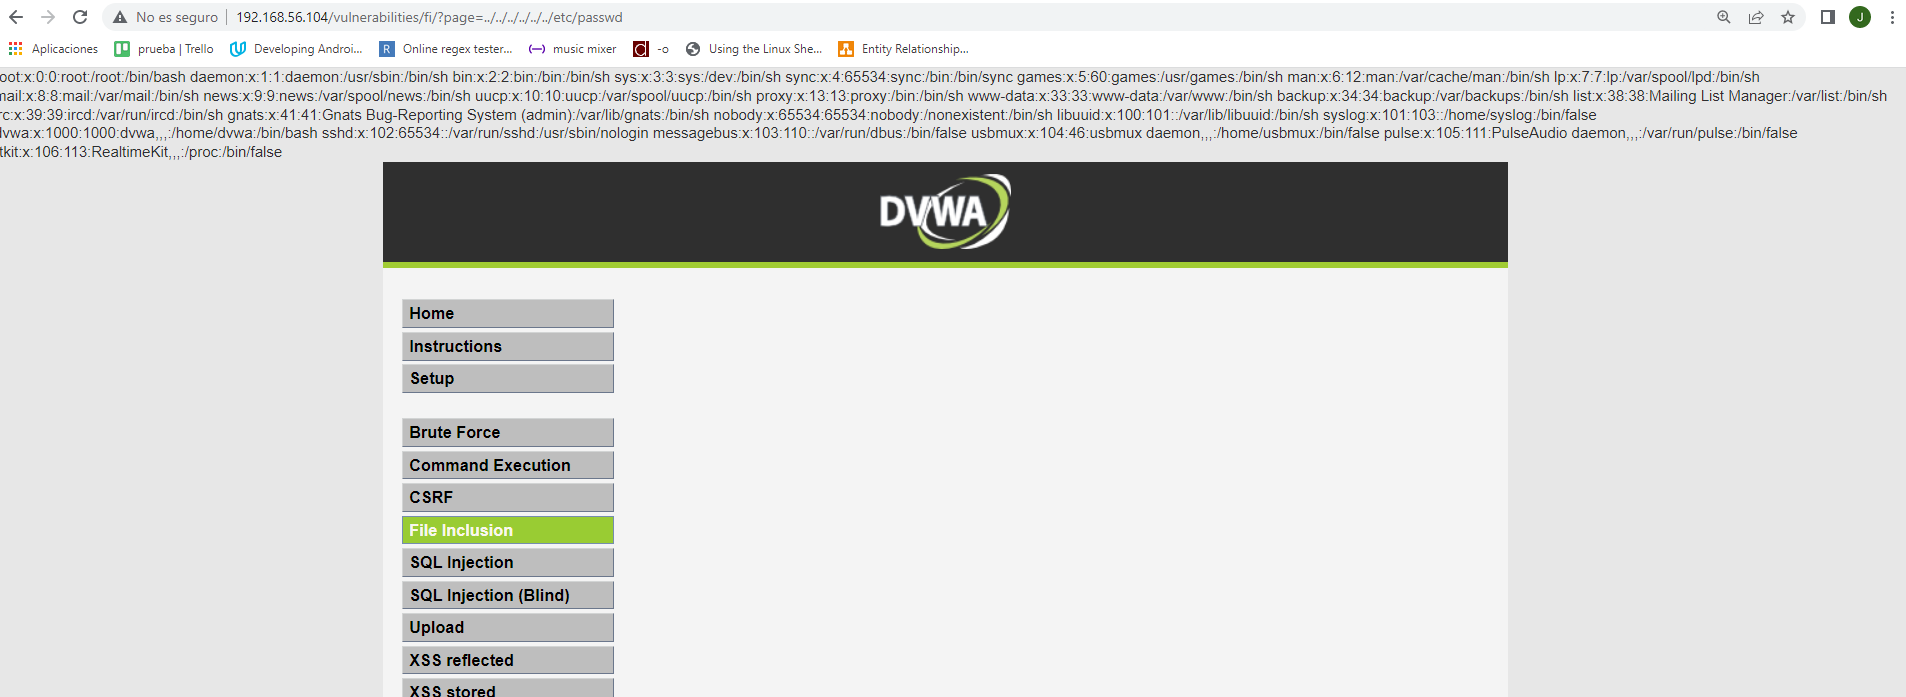
\includegraphics[scale=0.6]{fileUp1.png}
		\caption{}
		\label{fig:1}
	\end{figure}
	\newline \newline 
	Para el exploit en remoto, incluso en dificultad media es bastante sencillo ya que si vamos al codigo fuente, vemos que se filtra de la siguiente forma:
	\begin{figure}[!h]
		\centering
		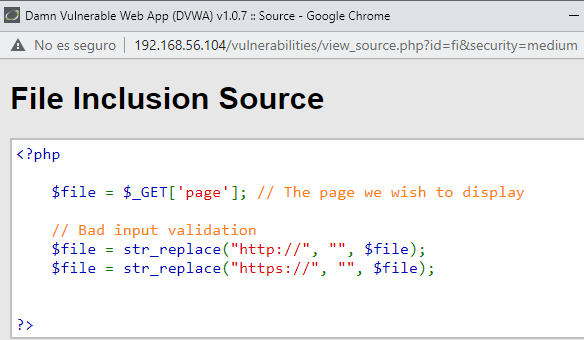
\includegraphics[scale=0.6]{fi1.png}
		\caption{}
		\label{fig:2}
	\end{figure}
	\newpage{}
    Por lo que podr\'iamos simplemente poner en may\'usculas el http para evitarlo:
    \begin{lstlisting}[language = html]
    ?page=HttP://marca.com
    \end{lstlisting}
    Como nos pide el enunciado, nos falta evadir en local file include los filtros de nivel medio. Al tener los filtros de la Figura 2, nos es facil ver que podemos acceder desde la ra\'iz con \emph{/etc/passwd}.
    
\end{document}